% 原书 p.178–p.187（PDF p.186–p.195）

% >>> p186
\section{环面区域（Toric Domains）}

\begin{keytakeaways}
\begin{itemize}
  \item 几何图像：环面区域 $X_\Omega=\mu^{-1}(\Omega)$ 完全由平面区域
        $\Omega\subset\R^n_{\ge0}$（矩映射像）决定；$\Omega$ 的轮廓曲线承载了
        $X_\Omega$ 的全部定量信息，维数从 $2n$ 降到 $n$。
  \item 核心工具：Reeb 向量场的显式公式 (7.12)；闭 Reeb 轨道与法向量有理斜率
        判据（命题 7.2.1）；周期公式（命题 7.2.2）；单调性定义 7.2.2。
  \item 关键定理：定理 7.2.1（[42,63]）给出辛凸性的定量判据
        $c\le(a+b)\sqrt{T_{\min}}\le C$；定理 7.2.2（[109]）证明严格单调环面
        区域上一切球归一化容量都相等，从而 Viterbo 容量猜想（猜想 6.4.1）在此
        成立。
  \item 本节结论：环面凹/凸的命名与轮廓曲线的凸/凹恰好相反（原文如此）；单调性
        是排除嵌入的有力判据，也是 7.3 节形状不变量的背景。
\end{itemize}
\end{keytakeaways}

星形（或刘维尔）区域 $U\subset\C^n$ 是个复杂的对象，迄今我们只引入了辛同调
（见 6.3 节）作为研究 $U$ 的系统方法。然而，对 $\C^n$ 中一类特殊的 $U$——环面
区域——人们可以获得多得多的显式信息。它可以视为 2.5 节定义 2.5.2 中辛环面流形的
「开」类比。与 Arnold--Liouville 定理（见定理 2.8.1）类似，环面区域的内部是一个
以同一环面 $\T^n$ 为纤维的、（开）区域上的平凡纤维丛。更严格地说，借助矩映射
（见例 2.5.2）
\begin{equation}\tag{7.9}
  \mu\colon\C^n\to\R^n_{\ge0},\qquad
  (z_1,\dots,z_n)\mapsto(|z_1|^2,\dots,|z_n|^2),
\end{equation}
我们可以给出如下定义。

\begin{wdefn}{7.2.1}
  设 $X_\Omega\subset\C^n$ 是 $\C^n$ 中的一个区域。若它可写成 $\mu^{-1}(\Omega)$
  的形式，其中 $\mu$ 是 (7.9) 中的矩映射，而 $\Omega\subset\R^n_{\ge0}$ 是包含
  $\R^n_{\ge0}$ 中原点某邻域的闭区域，则称 $X_\Omega$ 是一个\textbf{环面区域}
  （toric domain）。区域 $\Omega$ 称为该环面区域的\textbf{矩映射像}
  （moment image）。
\end{wdefn}

% [Tutor Note: 术语依据——"toric domain" 译「环面区域」，"moment image" 译
% 「矩映射像」（与 2.4 节「矩映射」的译法保持一致）。注意两处容易出错：(i) $\mu$
% 的像落在 $\R^n_{\ge0}$ 而非整个 $\R^n$，所以 $\Omega$ 必须在 $\R^n_{\ge0}$ 中
% 含有原点邻域，否则 $\mu^{-1}(\Omega)$ 可能没有内点甚至不是区域；(ii) 这里
% 「开类比」是相对于紧的辛环面流形而言：$X_\Omega$ 通常非紧，其边界 $\partial
% X_\Omega$ 是切触流形。]

\begin{wexam}{7.2.1}
  辛椭球 $E(a_1,\dots,a_n)\in\C^n$（见 (3.7)）是 $\C^n$ 中的环面区域，其矩映射
  像是如下单纯形
  \[
    \Omega=\left\{(x_1,\dots,x_n)\in\R^n_{\ge0}\ \middle|\
    \frac{x_1}{a_1}+\cdots+\frac{x_n}{a_n}\le 1\right\}.
  \]
  特别地，$E(a,b)=X_\Omega$，其中 $\Omega$ 如图 7.2 所示。考虑另一个 $\Omega$，
  即图 7.3 中的矩形，则
  \begin{equation}\tag{7.10}
    X_\Omega=\{(z_1,z_2)\in\C^2\mid |z_1|^2\le a\ \text{且}\ |z_2|^2\le b\}
    =:P(a,b),
  \end{equation}
  称为\textbf{多圆盘}（polydisk）。注意在 $\Omega$ 的角点处，边界流形
  $\partial P(a,b)$ 不光滑。\hfill$//$
\end{wexam}

% >>> p187
\begin{figure}[htbp]
  \centering
  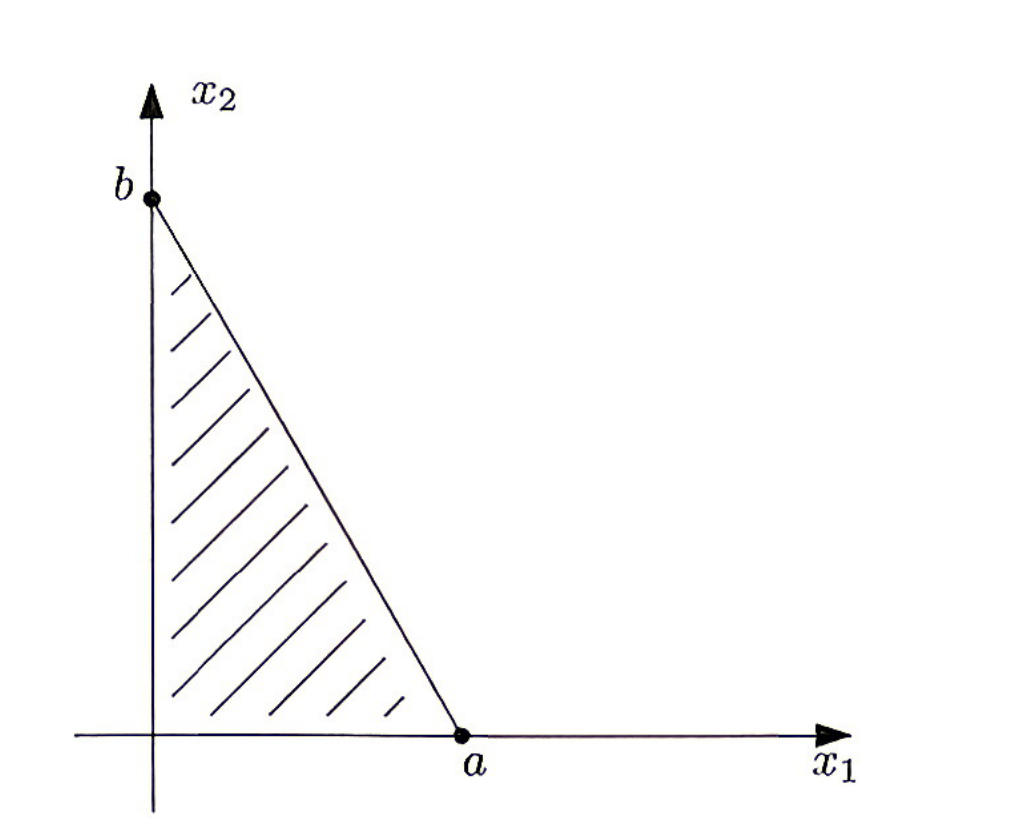
\includegraphics[width=0.62\linewidth]{figures/fig_p187_1.png}
  \caption*{图 7.2\quad $E(a,b)$ 的矩映射像（原书 p.179, Figure 7.2；PDF p.187）}
\end{figure}

\begin{figure}[htbp]
  \centering
  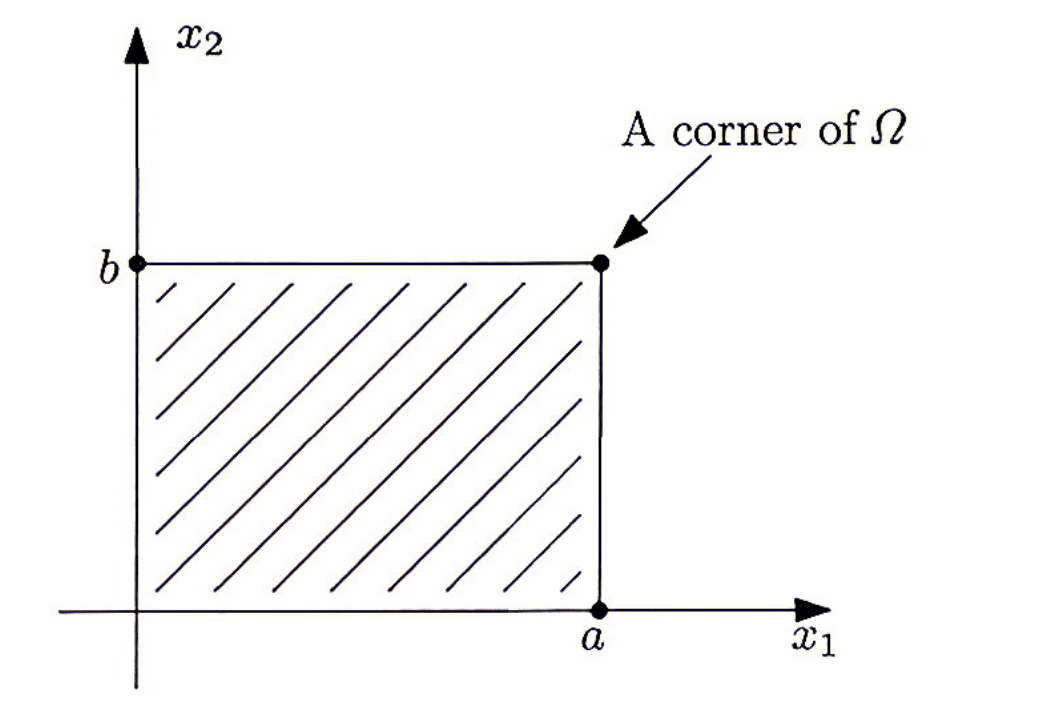
\includegraphics[width=0.62\linewidth]{figures/fig_p187_2.png}
  \caption*{图 7.3\quad $P(a,b)$ 的矩映射像（原书 p.179, Figure 7.3；PDF p.187）}
\end{figure}

接下来我们主要关注四维情形，即 $X_\Omega\subset\C^2$。人们可能会问：$X_\Omega$
何时是星形的（或刘维尔的）（见例 3.2.3）？可以快速验证：$X_\Omega$ 是星形的，
当且仅当 $\R^2_{\ge0}$ 中任一射线与 $\Omega$ 的轮廓曲线（即
$\overline{\partial\Omega\cap\R^2_{\ge0}}$）横截相交。换言之，$X_\Omega$ 的这一
几何性质可以直接从矩映射像 $\Omega$ 看出。仍由例 3.2.3，对任何星形 $X_\Omega$，
其边界 $\partial X_\Omega$ 是切触流形，切触结构由
$\ker(\lambda_{\mathrm{std}}|_{\partial X_\Omega})$ 给出。这里有一个自然的问题。

% >>> p188
\begin{wque}{7.2.1}
  我们能否直接从矩映射像 $\Omega$ 检测 $\partial X_\Omega$ 上的闭 Reeb 轨道，
  并读出它们的周期？
\end{wque}

让我们现在就开始计算。首先考虑环面区域 $\Omega$（见图 7.4）。固定任意点
$p=(p_1,p_2)\in\overline{\partial\Omega\cap\R^2_{\ge0}}$，其中
$p\ne(a,0)$ 或 $(0,b)$，并考虑 $\C^2$ 的极坐标
$(x_1,\theta_1,x_2,\theta_2)$——如前，$x_i=|z_i|^2$，$\theta_i\in[0,2\pi)$，
$i=1,2$（从而 $x_i(p)=p_i$，$i=1,2$）。则
$\omega_{\mathrm{std}}=\dd\lambda_{\mathrm{std}}$，其中
\[
  \lambda_{\mathrm{std}}=\frac{1}{2}x_1\,\dd\theta_1
  +\frac{1}{2}x_2\,\dd\theta_2.
\]
对任意 $z\in\mu^{-1}(p)$，可以验证
\begin{equation}\tag{7.11}
  T_z\partial X_\Omega
  =\left\{\sum_{i=1}^2a_i\frac{\partial}{\partial x_i}
  +b_i\frac{\partial}{\partial\theta_i}\ \middle|\
  a_i,b_i\in\R,\ \nu_1(p)a_1+\nu_2(p)a_2=0\right\}.
\end{equation}
这里 $(\nu_1(p),\nu_2(p))$ 是轮廓曲线在 $p$ 处的单位法向量。事实上，在
$\mu^{-1}(p)$ 附近，边界 $\partial X_\Omega$ 可视为 $\C^2$ 中由水平集
$\{F=0\}$ 给出的子流形。局部地，
$F(x_1,\theta_1,x_2,\theta_2)=h(x_1)-x_2$，其中 $h$ 是局部描述轮廓曲线的函数。
于是 $T_z\partial X_\Omega=\ker(\dd F(z))$。此外，
\[
  \dd F(z)=h'(x_1)\,\dd x_1+0\cdot\dd\theta_1
  -1\cdot\dd x_2+0\cdot\dd\theta_2.
\]
假设 $X=a_1\partial_{x_1}+b_1\partial_{\theta_1}+a_2\partial_{x_2}
+b_2\partial_{\theta_2}$，则 $\dd F(z)(X)=0$ 等价于
$-a_1h'(x_1)+a_2=0$。因此 $b_1,b_2$ 任意，而 $a_1,a_2$ 可取 $a_1=1$、
$a_2=h'(x_1)$。由于轮廓曲线在 $p$ 处的切向量是 $(1,h'(p))$，其法向量为
$(-h'(p),1)$，因此
\[
  (\nu_1(p),\nu_2(p))
  =\left(\frac{-h'(p)}{\sqrt{1+(h'(p))^2}},
  \frac{1}{\sqrt{1+(h'(p))^2}}\right).
\]

\begin{figure}[htbp]
  \centering
  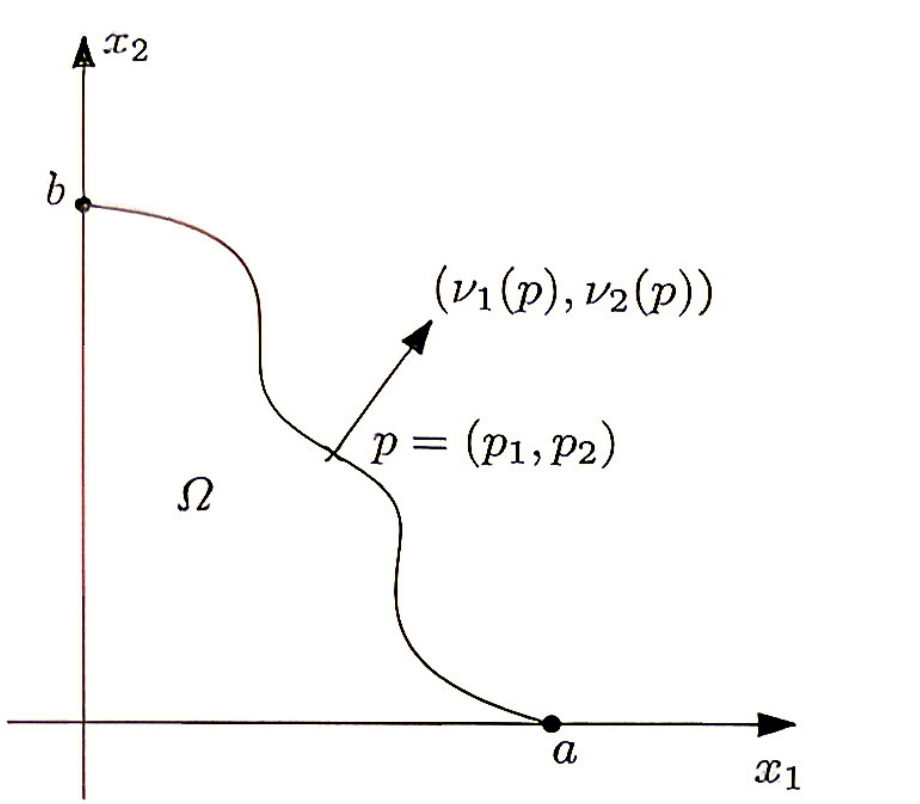
\includegraphics[width=0.56\linewidth]{figures/fig_p188_1.png}
  \caption*{图 7.4\quad $p$ 处的法向量（原书 p.180, Figure 7.4；PDF p.188）}
\end{figure}

% >>> p189
下面考虑 $\partial X_\Omega$ 上的 Reeb 向量场 $R_\alpha$，其中
$\alpha:=\lambda_{\mathrm{std}}|_{\partial X_\Omega}$。按定义有 $\alpha(R_\alpha)=1$
且 $\iota_{R_\alpha}\dd\alpha=0$。由 (7.11) 与 $\lambda_{\mathrm{std}}$ 的形式，
可以验证 $R_\alpha$ 是 $\xi(\nu_1(p)\partial/\partial\theta_1
+\nu_2(p)\partial/\partial\theta_2)$ 的倍数（其中 $\xi$ 为某函数），即
\begin{equation}\tag{7.12}
  R_\alpha(z)=\frac{2}{\nu_1(p)p_1+\nu_2(p)p_2}
  \left(\nu_1(p)\frac{\partial}{\partial\theta_1}
  +\nu_2(p)\frac{\partial}{\partial\theta_2}\right).
\end{equation}
确实，$R_\alpha(z)\in T_z\partial X_\Omega$，因为它在
$\partial/\partial x_i$ 方向上没有分量。按定义（见 (3.2)），$\alpha(R_\alpha)=1$
的验证由如下计算得到：
\[
  \begin{aligned}
    &\left(\frac12x_1(p)\,\dd\theta_1+\frac12x_2(p)\,\dd\theta_2\right)\\
    &\qquad\left(\frac{2}{\nu_1(p)p_1+\nu_2(p)p_2}
    \left(\nu_1(p)\frac{\partial}{\partial\theta_1}
    +\nu_2(p)\frac{\partial}{\partial\theta_2}\right)\right)
    =\frac{\nu_1(p)p_1+\nu_2(p)p_2}{\nu_1(p)p_1+\nu_2(p)p_2}=1.
  \end{aligned}
\]
此外，$\iota_{R_\alpha}\dd\alpha=0$ 的验证可由如下计算得到：
\begin{align*}
  &\left(\frac12\dd x_1\wedge\dd\theta_1
  +\frac12\dd x_2\wedge\dd\theta_2\right)
  \left(\frac{2}{\nu_1(p)p_1+\nu_2(p)p_2}
  \left(\nu_1(p)\frac{\partial}{\partial\theta_1}
  +\nu_2(p)\frac{\partial}{\partial\theta_2}\right),\cdot\right)\\
  &\qquad=\frac{1}{\nu_1(p)p_1+\nu_2(p)p_2}
  \bigl(\nu_1(p)\,\dd x_1+\nu_2(p)\,\dd x_2\bigr).
\end{align*}
对任意 $w\in T_z\partial X_\Omega$，由 (7.11)，$w$ 在分量 $\partial_{x_1}$ 与
$\partial_{x_2}$ 前的两个系数 $a_1$ 与 $a_2$ 分别满足
$\nu_1(p)a_1+\nu_1(p)a_2=0$。因此，作为 1-形式的
$\iota_{R_\alpha}\dd\alpha$ 在任意 $w\in T_z\partial X_\Omega$ 上总是消失，正如
所要求的那样。

% [Tutor Note: 原文疑误——上式 $\nu_1(p)a_1+\nu_1(p)a_2=0$ 中的第二个
% $\nu_1(p)$ 应为 $\nu_2(p)$：由 (7.11) 直接读出的是
% $\nu_1(p)a_1+\nu_2(p)a_2=0$，否则下一句「$\iota_{R_\alpha}\dd\alpha$ 总是
% 消失」不成立。此处保留原文写法，已记入审校记录。]

\begin{wrem}{7.2.1}
  一个重要的观察是：由 (7.12) 可知，Reeb 向量场总落在同一个纤维环面
  $\mu^{-1}(p)$ 中。
\end{wrem}

有了上述讨论，我们就能相当精确地刻画 $\partial X_\Omega$ 上的闭 Reeb 轨道，这
总结为下述命题。

\begin{wprop}{7.2.1}
  设 $X_\Omega$ 是 $\C^2$ 中的星形环面区域。假设矩映射像 $\Omega$ 的边界
  $\overline{\partial\Omega\cap\R^2_{\ge0}}$ 是光滑的。则对某个
  $p\in\overline{\partial\Omega\cap\R^2_{\ge0}}$，记作 $\gamma_p$ 的闭 Reeb 轨道
  出现在纤维环面 $\mu^{-1}(p)$ 中，当且仅当（单位）法向量方向
  $(\nu_1(p),\nu_2(p))$ 满足 $\nu_2(p)/\nu_1(p)\in\Q$。此外，曲线
  $\overline{\partial\Omega\cap\R^2_{\ge0}}$ 与 $\R^2_{\ge0}$ 两条坐标轴的两个
  交点也对应于两条闭 Reeb 轨道，它们分别位于辛平面 $\C\times\{0\}$ 与
  $\{0\}\times\C$ 中。
\end{wprop}

\begin{wproof}
  由 (7.12)，$R_\alpha$ 的流是闭轨道，当且仅当系数 $\nu_1(p)$ 与 $\nu_2(p)$ 之比
  为有理数。
\end{wproof}

\begin{wexam}{7.2.2}
  对四维椭球 $E(a,b)$，若 $\dfrac{b}{a}\notin\Q$，则对任何
  $p\in\overline{\partial\Omega\cap\R^2_{\ge0}}$ 都有
  $\nu_2(p)/\nu_1(p)=a/b$ 恒为无理数。因此，仅有的 2 条单的（或本原的）闭 Reeb
  轨道就是来自坐标轴交点的两条，即例 3.2.3 末尾所定义的 $\gamma_a$ 与
  $\gamma_b$。\hfill$//$
\end{wexam}

% >>> p190
\begin{wexam}{7.2.3}
  对 (7.10) 中的多圆盘 $P(a,b)$，在把其矩形矩映射像的右上角顶点 $(a,b)$
  光滑化之后（见图 7.5），由命题 7.2.1，我们将得到无穷多条单闭 Reeb 轨道，因为
  当我们从左向右靠近光滑化的角点时，斜率 $\nu_2(p)/\nu_1(p)$ 会从 $+\infty$
  变回 $0$。\hfill$//$
\end{wexam}

\begin{figure}[htbp]
  \centering
  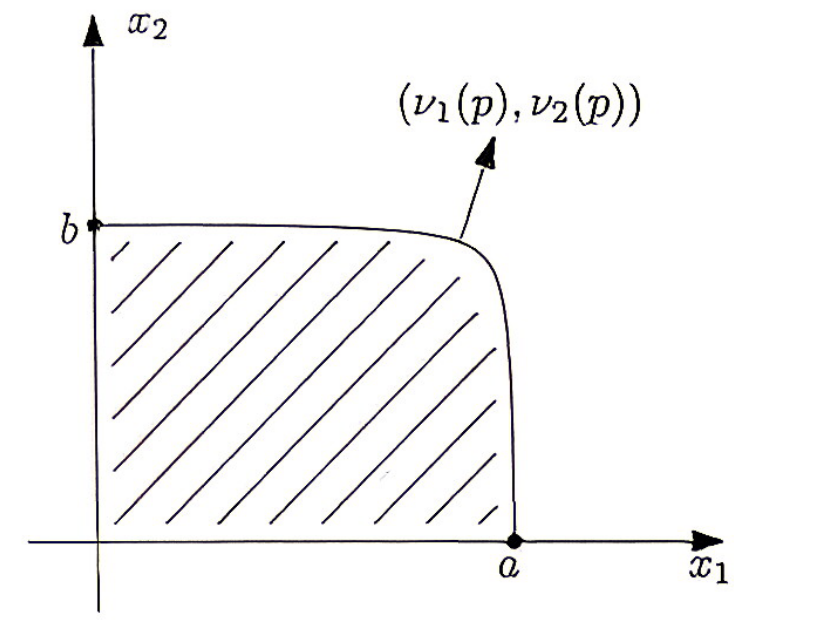
\includegraphics[width=0.58\linewidth]{figures/fig_p190_1.png}
  \caption*{图 7.5\quad $\Omega$ 光滑化角点处的闭轨道（原书 p.182, Figure 7.5；
    PDF p.190）}
\end{figure}

设 $p$ 满足 $(\nu_2(p)/\nu_1(p))\in\Q$。由命题 7.2.1，在 $\mu^{-1}(p)$ 中存在
一条单闭 Reeb 轨道，记作 $\gamma_p$。关于 $\gamma_p$ 的一项重要信息是它的周期
（或作用量——见练习 5.4.1）。事实上，由 (7.12)，它是使
\begin{equation}\tag{7.13}
  (\lambda_p\nu_1(p),\lambda_p\nu_2(p))\in\Z^2
\end{equation}
成立的最小正实数，记作 $\lambda_p$。特别地，$\lambda_p\nu_1(p)$ 与
$\lambda_p\nu_2(p)$ 互素（这对应于该闭 Reeb 轨道是单的）。$\gamma_p$ 到
$\theta_i$-平面的投影将是一条被绕行 $\lambda_p\nu_i(p)$ 次的圆周，$i=1,2$。
于是下述命题是直接的。

\begin{wprop}{7.2.2}
  设 $X_\Omega$ 是 $\C^2$ 中的星形环面区域，$p\in\partial\Omega\cap\R^2_{\ge0}$
  满足 $(\nu_2(p)/\nu_1(p))\in\Q$。又设 $\gamma_p$ 是纤维环面 $\mu^{-1}(p)$ 中
  的单闭 Reeb 轨道。则其周期（由 $\int_{\gamma_p}\alpha$ 定义）等于
  \[
    p_1\lambda_p\nu_1(p)+p_2\lambda_p\nu_2(p)
    \ \bigl(=(p_1,p_2)\cdot(\lambda_p\nu_1(p),\lambda_p\nu_2(p))\bigr),
  \]
  即位置向量 $(p_1,p_2)$ 与重新标度后的法向量
  $(\lambda_p\nu_1(p),\lambda_p\nu_2(p))$ 的内积。此外，对来自坐标轴交点的单闭
  Reeb 轨道，其周期是对应交点的截距乘以 $\pi$。
\end{wprop}

% [Tutor Note: 含糊点拨——命题 7.2.2 后半句「来自坐标轴交点的轨道，周期为截距
% 乘以 π」无法由 (7.12) 直接读出：在 $p=(a,0)$ 或 $(0,b)$ 处法向量退化为
% $(1,0)$ 或 $(0,1)$，纤维环面 $\mu^{-1}(p)$ 退化为圆周，Reeb 场沿
% $\partial/\partial\theta_i$ 方向。此时 $\alpha=\frac12x_i\,\mathrm{d}\theta_i$、
% $\alpha(R_\alpha)=1$ 给出 $R_\alpha=\frac{2}{x_i}\partial_{\theta_i}$，故周期
% $=2\pi\cdot\frac{x_i}{2}=\pi x_i$。核对时请勿把 (7.12) 的因子 $2$ 与周期公式
% 混用。]

为简化叙述，我们称曲线 $\overline{\partial\Omega\cap\R^2_{\ge0}}$ 为环面区域
$X_\Omega$ 的矩映射像 $\Omega$ 的\textbf{轮廓曲线}（profile curve）。按这条
曲线的形状，$\C^2$ 中有若干特殊的环面区域子族。

% >>> p191
\begin{wdefn}{7.2.2}
  (i) 若环面区域 $X_\Omega$ 的矩映射像 $\Omega$ 的轮廓曲线是凸曲线，则称
  $X_\Omega$ 是\textbf{环面凹的}（toric concave）（见图 7.6 第一幅图）。
  (ii) 若 $X_\Omega$ 的矩映射像的轮廓曲线是凹曲线，则称 $X_\Omega$ 是
  \textbf{环面凸的}（toric convex）（见图 7.6 第二幅图）。
  (iii) 若对矩映射像的轮廓曲线上任意点 $p$，外法向量
  $\nu=(\nu_1(p),\nu_2(p))$ 满足 $\nu_i(p)\ge0$（$i=1,2$），则称 $X_\Omega$ 是
  \textbf{单调的}（monotone）（见图 7.6 第三幅图）。进一步，若对轮廓曲线上
  任意点 $p$ 与 $i=1,2$ 都有 $\nu_i(p)>0$，则称单调环面区域 $X_\Omega$ 是
  \textbf{严格单调的}（strictly monotone）。
\end{wdefn}

% [Tutor Note: 易错预警——这是全章最易混淆的命名：环面凹（toric concave）的
% 轮廓曲线是凸曲线，环面凸（toric convex）的轮廓曲线反而是凹曲线。请对照图 7.6
% 记住「环面凹 = 区域边界向外鼓」。另注意 (iii) 中 $\nu_i(p)\ge0$ 是对外法向
% 而言：若把轮廓曲线写成 $x_2=h(x_1)$ 且 $h$ 递减，则 $h'<0$ 使
% $\nu_1=-h'/\sqrt{1+h'^2}>0$、$\nu_2=1/\sqrt{1+h'^2}>0$，故严格单调等价于
% $h'<0$（轮廓曲线严格递减）。]

\begin{figure}[htbp]
  \centering
  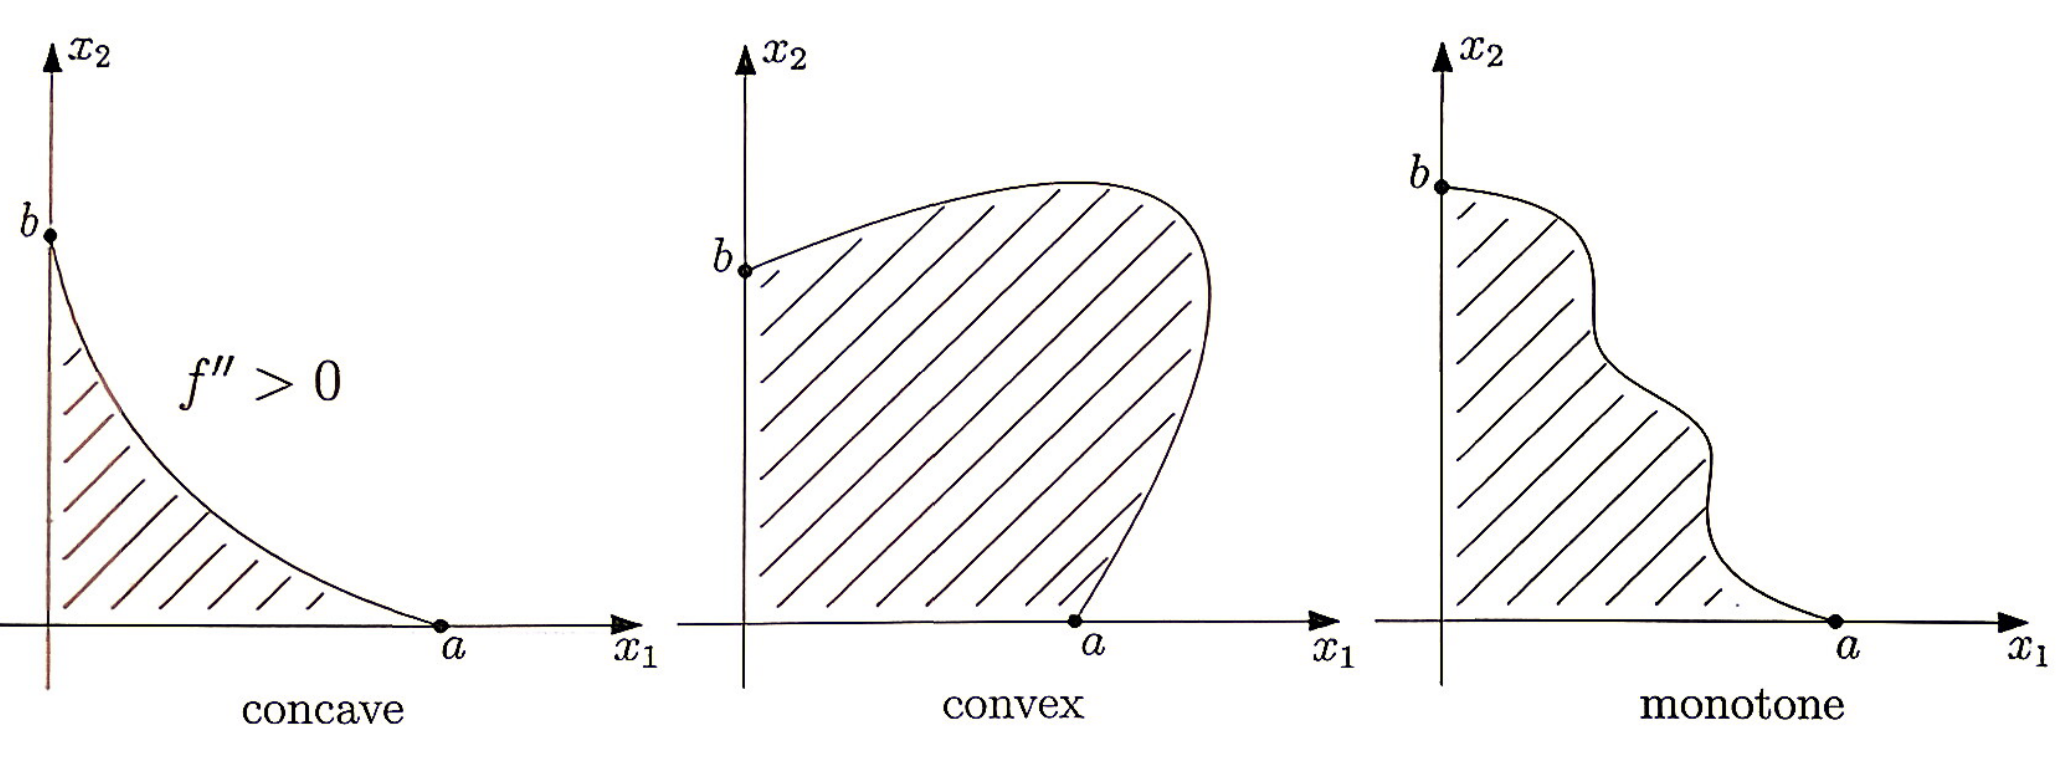
\includegraphics[width=0.95\linewidth]{figures/fig_p191_1.png}
  \caption*{图 7.6\quad $\C^2$ 中三族特殊的环面区域：环面凹（左）、环面凸（中）、
    单调（右）（原书 p.183, Figure 7.6；PDF p.191）}
\end{figure}

\begin{wexam}{7.2.4}
  由 (7.10) 定义的多圆盘 $P(a,b)$ 是单调环面区域（不是严格单调的，但是凸的）。
  四维椭球 $E(a,b)$ 是严格单调的；它同时既是凸的又是凹的。\hfill$//$
\end{wexam}

\begin{wexam}{7.2.5}
  给定严格单调环面区域，由初等几何，位置向量 $(p_1,p_2)$ 与重新标度后的法向量
  $(\lambda_p\nu_1(p),\lambda_p\nu_2(p))$ 的内积总是大于 $0$（见图 7.7）。因此，
  命题 7.2.2 表明：只要 $X_\Omega$ 是严格单调环面区域，$\partial X_\Omega$ 的
  所有闭 Reeb 轨道都有正的周期，即总是大于 $0$。\hfill$//$
\end{wexam}

有趣的是，矩映射像 $\Omega$ 的形状有时并\emph{不}反映环面区域 $X_\Omega$ 本身
的同一几何性质。下述练习说明了一例。

\begin{wexer}{7.2.1}
  (i) 设 $X_\Omega$ 是环面凹区域（见图 7.6 第一幅图），其轮廓曲线由
  $\R^2_{\ge0}$ 中的 $(x_1)^{2/3}+(x_2)^{2/3}=1$ 给出。证明 $X_\Omega$ 是
  $\C^2$ 中的一个（几何）凸区域（尽管矩映射像 $\Omega$ 不是 $\R^2_{\ge0}$ 的
  凸子集）。
  (ii) 一般地，证明 $X_\Omega$ 是 $\C^2$ 中的（几何）凸区域，当且仅当集合
  \[
    \sqrt{\Omega}:=\bigl\{(p_1,p_2)\in\R^2\ \big|\ (|p_1|^2,|p_2|^2)\in\Omega
    \bigr\}
  \]
  是 $\R^2$ 的凸子集。
\end{wexer}

% >>> p192
\begin{figure}[htbp]
  \centering
  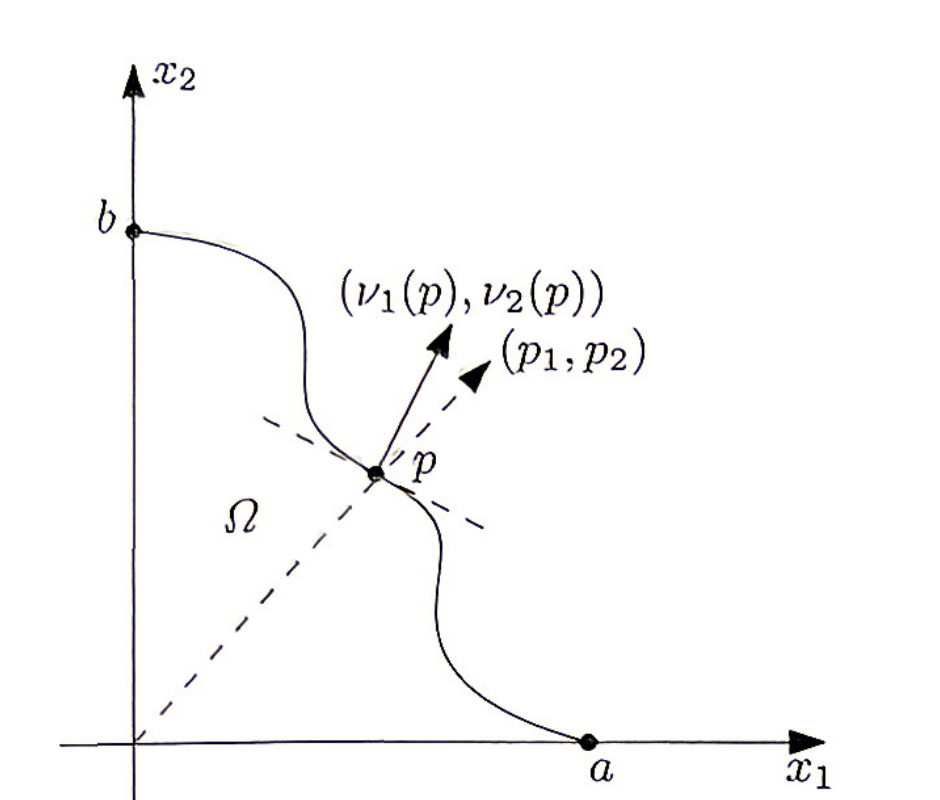
\includegraphics[width=0.56\linewidth]{figures/fig_p192_1.png}
  \caption*{图 7.7\quad 法向量 $(\nu_1(p),\nu_2(p))$ 与位置向量
    $p=(p_1,p_2)$（原书 p.184, Figure 7.7；PDF p.192）}
\end{figure}

承接上面的练习 7.2.1：研究环面区域 $X_\Omega$ 的（几何）凸性是有意义的，但需
稍加小心——它不是辛性质，即 $X_\Omega$ 的凸性可能在辛同胚作用下改变。为解决这一
问题，可以定义：若 $X_\Omega$ 在某个辛同胚下是（几何）凸的，则称 $X_\Omega$ 是
\textbf{辛凸的}（symplectically convex）。下面是一个颇令人好奇的问题：

\begin{wque}{7.2.2}
  任何（星形）环面区域 $X_\Omega$ 是否都是辛凸的？
\end{wque}

答案很快是否定的（而且确实存在大量非辛凸的环面区域），因为（几何）凸性在各种
意义上都是一种特殊的性质。例如，[122] 证明：若星形 $X_\Omega\subset\C^2$ 是
（几何）凸的，则与 $\partial X_\Omega$ 的任一闭 Reeb 轨道相关联的某版本
Conley--Zehnder 指标（见 5.5 节）必须至少为 $3$。任何满足这一指标条件的区域
都称为\textbf{动力凸的}（dynamically convex）。此外，动力凸性是一个辛性质；
因此，[122] 证明任何辛凸的 $X_\Omega$ 必是动力凸的。于是问题 7.2.2 可以修正为：
任何动力凸的 $X_\Omega$ 是否也是辛凸的？有趣的是，答案仍然是否定的！迄今为止，
至少有两种途径通过建立 $X_\Omega$ 辛凸的某些必要条件来确认这一点。下述定理就是
其中之一。

\begin{wthm}{7.2.1$^{[42,63]}$}
  存在常数 $c,C>0$，使得对任何星形环面区域 $X_\Omega\subset\C^2$，若其体积落在
  $(2-2\epsilon,2+2\epsilon)$ 中（$\epsilon>0$ 充分小），且 $X_\Omega$ 是辛凸的，
  则下述不等式成立：
  \begin{equation}\tag{7.14}
    c\le(a+b)(T_{\min})^{\frac12}\le C.
  \end{equation}
  这里 $a,b$ 分别是 $\Omega$ 的 $x_1$-截距与 $x_2$-截距，而 $T_{\min}$ 表示
  $\partial X_\Omega$ 中闭 Reeb 轨道的最小周期。
\end{wthm}

% >>> p193
在下述例子中，我们将看到如何通过扰动作为 $\C^2$ 中环面区域的辛球 $B^4(2)$
来应用定理 7.2.1。

\begin{wexam}{7.2.6}
  考虑一族环面区域 $X_{\Omega_\epsilon}$，其中 $\Omega_\epsilon$ 如图 7.8 所示，
  $\epsilon\to0$。我们将光滑化 $(\epsilon,\epsilon)$ 处的角点。由命题 7.2.1 与
  命题 7.2.2 易验证：当 $\epsilon$ 充分小时，$T_{\min}$ 由出现在纤维环面
  $\mu^{-1}((\epsilon,\epsilon))$ 处的单闭 Reeb 轨道给出，且等于
  $\epsilon\cdot1+\epsilon\cdot1=2\epsilon$。于是，当 $\epsilon$ 充分小时
  （此时 $a=b=2$），有
  \[
    (a+b)(T_{\min})^{\frac12}=4\cdot\sqrt{2\epsilon}<c,
  \]
  这违反定理 7.2.1 中的不等式 (7.14)。因此，当 $\epsilon\to0$ 时，
  $X_{\Omega_\epsilon}$ 不是辛凸的。\hfill$//$
\end{wexam}

\begin{figure}[htbp]
  \centering
  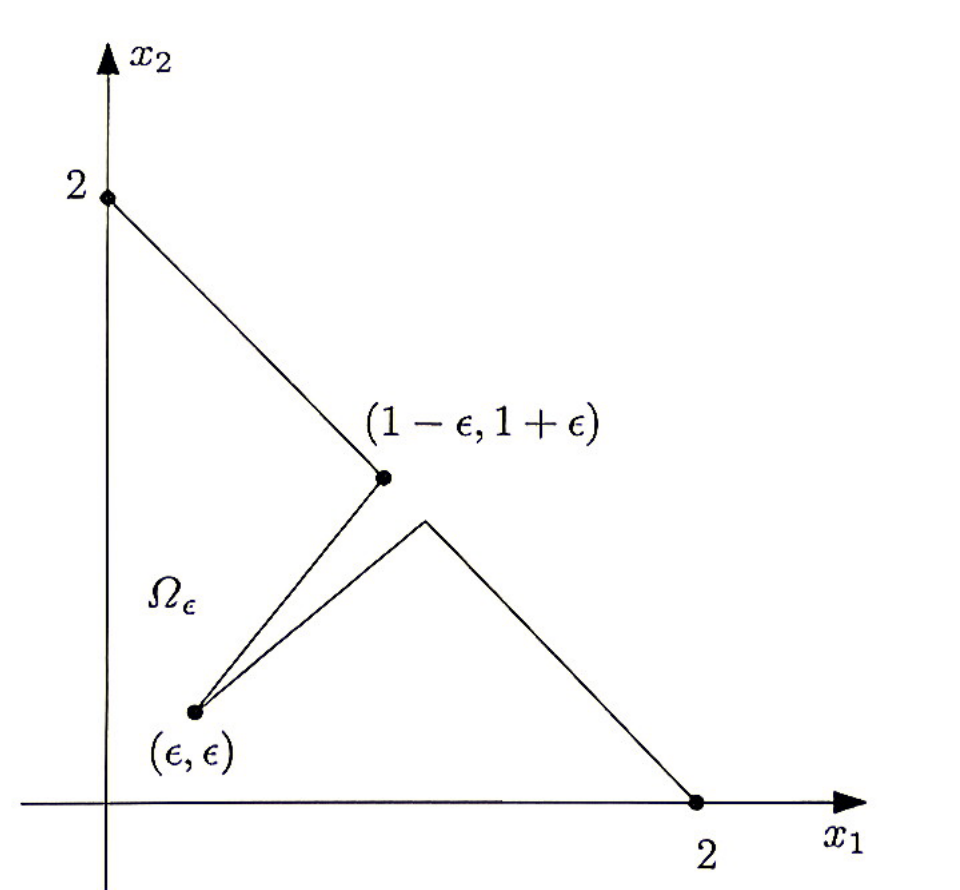
\includegraphics[width=0.58\linewidth]{figures/fig_p193_1.png}
  \caption*{图 7.8\quad 最小周期为 $2\epsilon$ 的非凸区域（原书 p.185,
    Figure 7.8；PDF p.193）}
\end{figure}

\begin{wexam}{7.2.7}
  考虑另一族环面区域 $X_{\Omega_\epsilon}$，其中 $\Omega_\epsilon$ 如图 7.9
  所示，$\epsilon\to0$。此时 $a+b=\dfrac1\epsilon+2\to+\infty$
  （当 $\epsilon\to0$）。同时可以验证 $T_{\min}$ 只在一个小范围内变化。因此，
  当 $\epsilon\to0$ 时，
  \[
    (a+b)(T_{\min})^{\frac12}
    =\left(\frac1\epsilon+2\right)\cdot(T_{\min})^{\frac12}>C,
  \]
  这违反定理 7.2.1 中的不等式 (7.14)。所以当 $\epsilon\to0$ 时，
  $X_{\Omega_\epsilon}$ 不是辛凸的。\hfill$//$
\end{wexam}

% >>> p194
\begin{figure}[htbp]
  \centering
  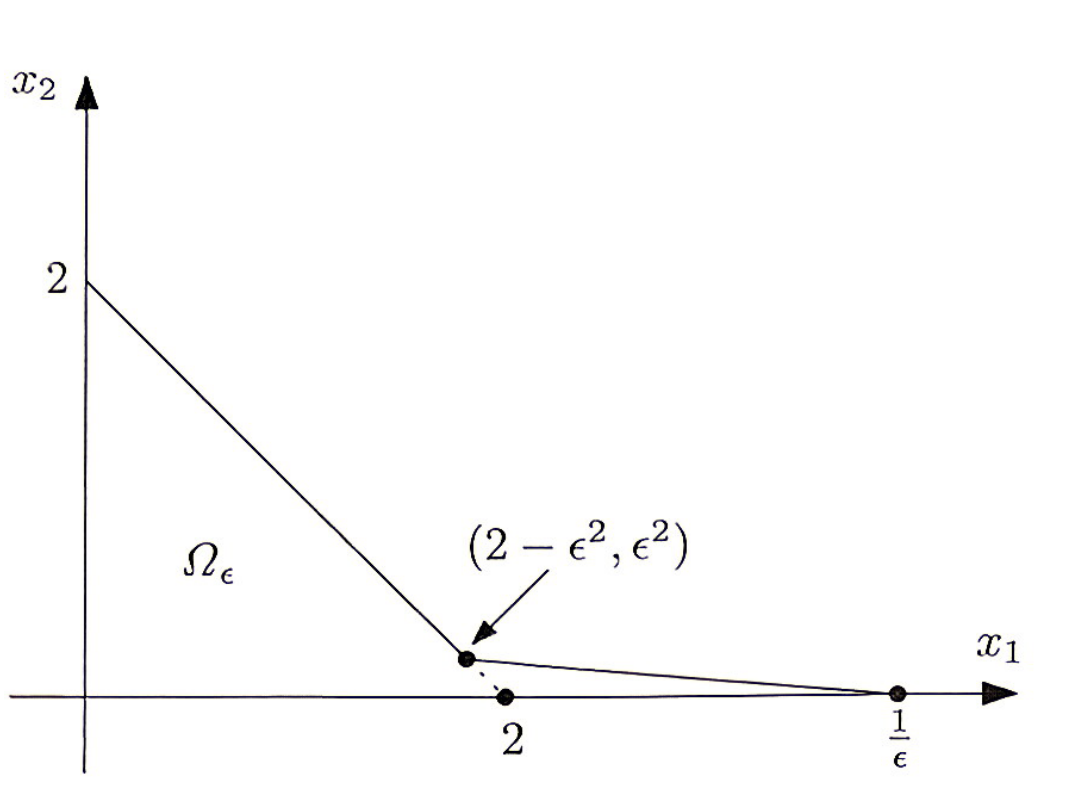
\includegraphics[width=0.62\linewidth]{figures/fig_p194_1.png}
  \caption*{图 7.9\quad $a+b\to+\infty$ 的非凸区域（原书 p.186, Figure 7.9；
    PDF p.194）}
\end{figure}

\begin{wrem}{7.2.2}
  事实上，例 7.2.6 中的环面区域族 $X_\Omega$ 是动力凸的。因此，它给出了动力凸
  但非辛凸区域的例子。
\end{wrem}

本节最后，我们提一下关于环面区域 $X_\Omega$ 严格单调性的下述定量刻画（作为必要
条件）。

\begin{wthm}{7.2.2（[109] 中的定理 1.7）}
  在任何严格单调环面区域 $X_\Omega\subset\C^2$ 上，所有球归一化容量都相等。
  因此，关于容量的 Viterbo 猜想（见猜想 6.4.1）在此情形下成立。
\end{wthm}

下面是证明的梗概。考虑能（通过包含映射）嵌入 $X_\Omega$ 内部的最大球
$B^4(r)$。由 Gromov 宽度 $w_G$ 的定义 (6.24)，我们知道 $w_G(X_\Omega)\ge r$。
由轮廓曲线严格递减的假设，代表 $B^4(r)$ 的等腰直角三角形的斜边与 $\Omega$ 的
轮廓曲线交于某点 $(x_1,x_2)$（从而 $x_1+x_2=r$）。见图 7.10。于是显然有
\[
  B^4(r)\subset X_\Omega\subset Z^4(x_1)\cup Z^4(x_2),
\]
其中 $Z^4(x_1)$ 与 $Z^4(x_1)$ 分别表示宽度为 $x_1$ 与 $x_2$ 的辛圆柱
（见 (1.13)）。关键一步是证明 $Z^4(x_1)\cup Z^4(x_2)$ 可辛嵌入 $Z^4(r)$。

% [Tutor Note: 原文疑误——本段原文 "where $Z^4(x_1)$ and $Z^4(x_1)$ denote
% symplectic cylinders with widths $x_1$ and $x_2$" 中第二个 $Z^4(x_1)$ 显系
% $Z^4(x_2)$ 之误：否则与 "widths $x_1$ and $x_2$"、图 7.10 以及
% $B^4(r)\subset X_\Omega\subset Z^4(x_1)\cup Z^4(x_2)$ 均矛盾。译文保留原文
% 写法并已记入审校记录。]

\begin{figure}[htbp]
  \centering
  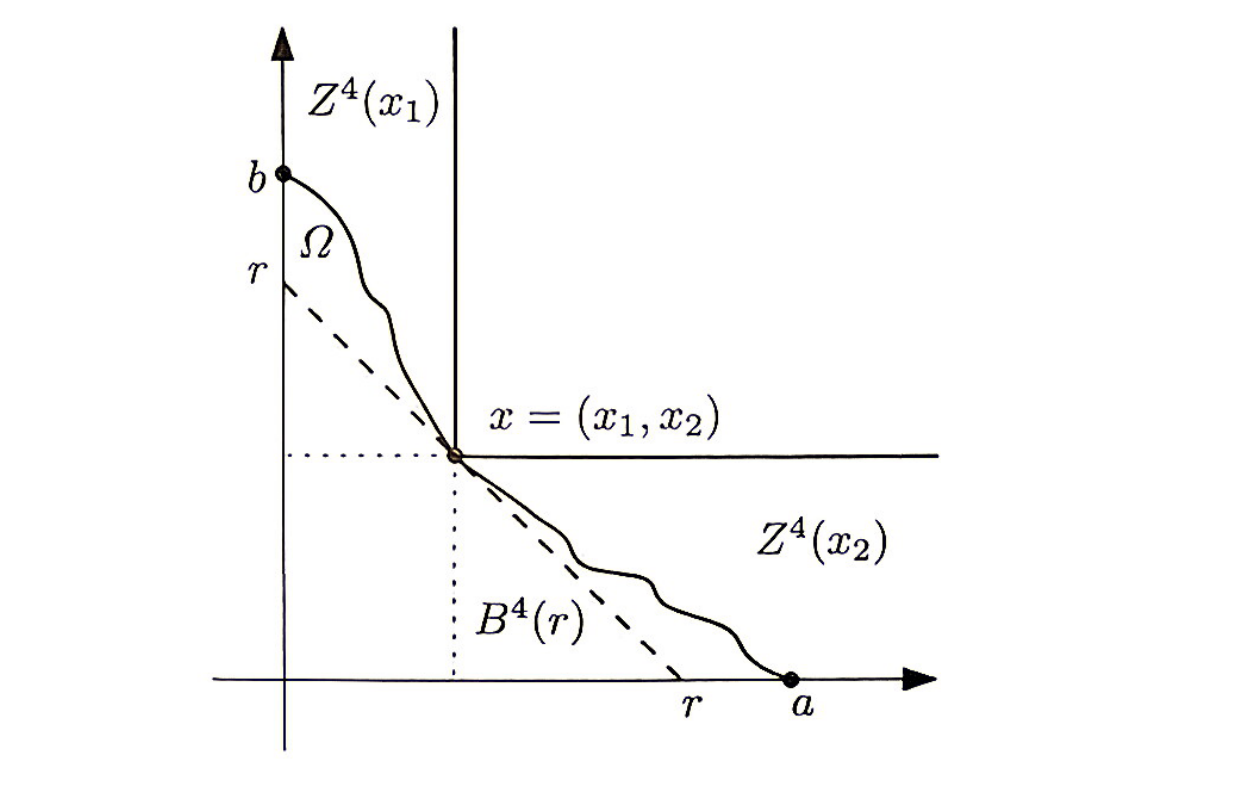
\includegraphics[width=0.62\linewidth]{figures/fig_p194_2.png}
  \caption*{图 7.10\quad $B^4(r)\hookrightarrow X_\Omega\hookrightarrow
    Z^4(x_1)\cup Z^4(x_2)$（原书 p.186, Figure 7.10；PDF p.194）}
\end{figure}

% >>> p195
对任何区域 $X\subset\C^2$，定义
\[
  c_Z(X):=\inf\{r\mid X\hookrightarrow Z^4(r)\}.
\]
则可以证明任何球归一化辛容量 $c$（见定义 6.4.1）满足 $c\le c_Z$
（参看练习 6.4.1）。因此，
\[
  r\le w_G(X_\Omega)\le c(X_\Omega)\le c_Z(X_\Omega)\le r,
\]
这说明对任何球归一化辛容量 $c$ 都有 $c(X_\Omega)=r$。

为证明辛嵌入 $Z^4(x_1)\cup Z^4(x_2)\hookrightarrow Z^4(r)$ 的存在性，我们可以
不显式构造所需的辛嵌入，而把问题转化为 $Z^4(x_1)\cup Z^4(x_2)$ 与 $Z^4(r)$ 的
ECH 容量（6.4 节引入）的比较。这是 [58] 中定理 1.2 的一个便利结果，它断言：
凹环面区域 $X_1$ 辛嵌入凸环面区域 $X_2$，当且仅当
\[
  c_k^{\mathrm{ECH}}(X_1)\le c_k^{\mathrm{ECH}}(X_2)
  \quad\text{对任何}\ k\in\N.
\]
幸运的是，$Z^4(x_1)\cup Z^4(x_2)$ 与 $Z^4(r)$ 都有 $c_k^{\mathrm{ECH}}$ 的
标准计算公式（见 [27]）。

\begin{wrem}{7.2.3}
  单调环面区域的概念、定理 7.2.1 中的判据以及定理 7.2.2 的结论，都已被 [43] 与
  [62] 成功地推广到更高维情形。
\end{wrem}
